\chapter{Method of work}
\label{chap:method}
\drop{I}{n} this chapter, the development software metodology during the
development of Geo-Cloud is described. Also, the tools such hardware and software used for is depicted.
 
\section{Development Metodology}
The selected metodology has been the \emph{iterative and incremental}
model. This model provides numerous advantages as early adaptability, testing
continously and to have a implementation quite close to the final product. A
scheme of the model is shown in figure~\ref{fig:IncrementalModel}.


\begin{figure}[!h]
\begin{center}
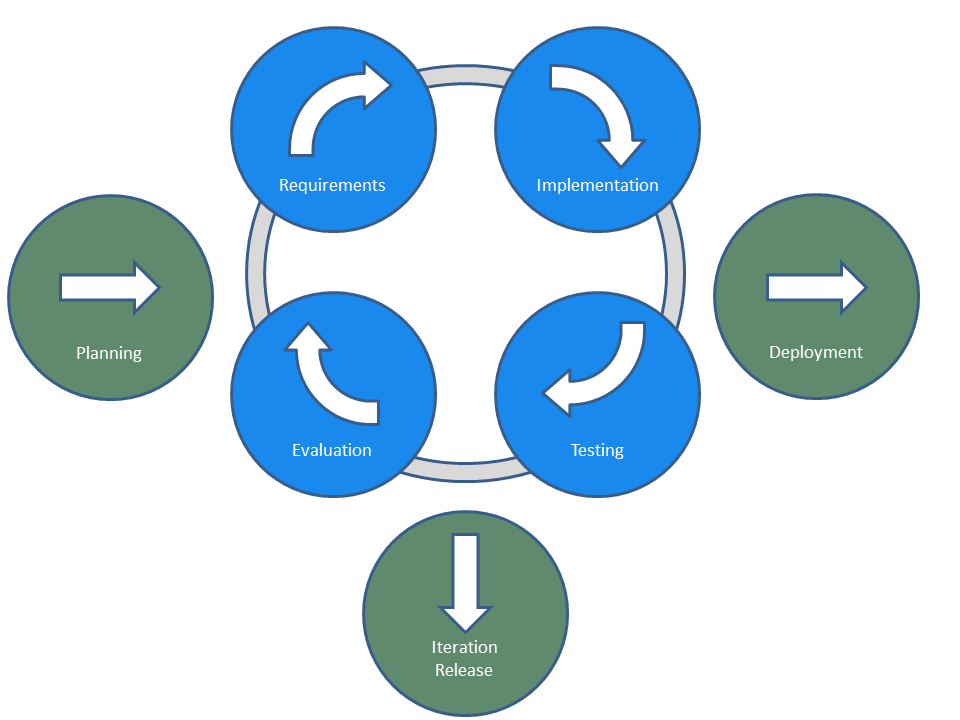
\includegraphics[width=0.7\textwidth]{statement/IterativeIncrementalDevelopment.png}
%http://www.meranetworks.com/services/processes/iterative
\caption{Iterative-incremental model}
\label{fig:IncrementalModel}
\end{center}
\end{figure}

This metodology enforces a strategy based in small iterations in which ones
there are short changes applies to each module. This permits to generate a prototype
growing and closing to the final version validating the initial requirements. In
this way if any changes are required by the advisor, is easilly to carry out
them.
 
As the project has several parts, it is divided in modules and simultaneosly,
each module is divided in iterations. This iterations are depicted in section XXXX.

\section{Tools}

In this section the resources such software and hardware used during the
developement are enumerated and described.  



\subsection{Programming Languages}

Several programming languages have been used for the Geo-Cloud
implementation. These languages are the following:

\begin{itemize}
\item \textbf{Python:} lenguaje principal usado en el proyecto. Se ha elegido
  Python debido a la posibilidad de ejecución sin necesidad de compilarlo ya que
  en BonFIRE las máquinas son distintas; por ser multiplataforma; cuenta con
  numerosas librerías que permiten hacer de este lenguaje un lenguaje dinámico y
  además es un lenguaje sencillo y muy ágil.

  Main language used in the project. It has been selected ought to it is not
  necessary to compile the source (the operative systems in the cloud may be not
  the same); it is a multiplatform language; it has lots of libraries in order
  to achive any purpouse.
 \item \textbf{XML:} It is used in some configuration files used by the
   Orchestrator module or the User Interface tool.

\item \textbf{Json:} The BonFIRE experiment descriptor must be writted in this
  language indicating the virtual machines instances, physical machines and the
  network resources instantiated.

\item \textbf{Bash:} Language used for doing some scripts. 

\end{itemize}


\subsection{Hardware}

The development of Geo-Cloud project has been carried out in a PC owned by
Deimos with the following features:
\begin{itemize}
\item \emph{Intel Core i5 3450 3.1 GHz}
\item \emph{8 GB RAM}
\end{itemize}

For the Version Control, the chosen server is
Bitbucket~\footnote{http:www.bitbucket.org}.

The used resources provided  by the Fed4FIRE testbeds are the following:

\begin{itemize}
\item \textbf{PlanetLab}: It currently provides 1204 nodes at 593 sites arround
  the world. 50 nodes have been used for to carry out the PlanetLab experiment.

\item \textbf{Virtual Wall}: It consists of 100 nodes (dual processor o dual
  core servers) interconnected via a non-blocking 1.5 Tb/s Ethernet switch. 29
  nodes have been used to simulate the satellite constellation and ground
  stations. \emph{PONER LO DE LAS METRICAS E IMPAIRMENTS}

\item \textbf{BonFIRE}: Nodes from diferent testbeds have been selected:
  \begin{itemize}
    \item From Inria: 2 nodes Medium : 

\end{itemize}
\end{itemize}

\emph{Explain the BonFIRE hardware???}

\subsection{Software}

Then, the tools and libraries used for the project are depicted:

\begin{itemize}
\item \textbf{Operative Systems}
\begin{itemize}
\item{\emph{Ubuntu}}: the operative system in which the development has done.
\item{\emph{Debian}}: the BonFIRE, Virtual Wall and PlanetLab machines run this operative system.
\end{itemize}
\item \textbf{Software Development Tools}

\begin{itemize}
\item{\emph{Emacs}}: versatile and powerfull text editor developed by Richard
  Stallman. This tool is used with pymacs together. Used version 23.2.
\item{\emph{JFed}}: tool developed by IMinds (University of Gent)\footnote{http:www.jfed.iminds.be}
\item{\emph{BonFIRE Web Interface}}: BonFIRE tool that provides the experiment
  deployment manually or to upload a experiment descriptor for automatic deployment.
\end{itemize}


\item \textbf{Graphics and documentation}

\begin{itemize}
\item{\emph{\LaTeX}}: versatile and powerfull text editor developed by Richard
  Stallman. This tool is used with pymacs together. Used version 23.2.
\item{\emph{GIMP}}: tool developed by IMinds (University of Gent)\footnote{http:www.jfed.iminds.be}
\item{\emph{Dia}}: BonFIRE tool that provides the experiment
  deployment manually or to upload a experiment descriptor for automatic deployment.
\item{\emph{UmlLet}}: BonFIRE tool that provides the experiment

\end{itemize}

\item \textbf{Software Libraries}

\begin{itemize}
\item{\emph{python-mysql}}: versatile and powerfull text editor developed by Richard
  Stallman. This tool is used with pymacs together. Used version 23.2.
\item{\emph{python-mathplotlib}}: tool developed by IMinds (University of Gent)\footnote{http:www.jfed.iminds.be}
\item{\emph{python-xml}}: BonFIRE tool that provides the experiment
  deployment manually or to upload a experiment descriptor for automatic deployment.
\item{\emph{paramiko}}:Tobe defined

\end{itemize}
...more
\end{itemize}
